Il \textit{Data Analyzer} si occupa dell'analisi dei dati raccolti dal \textit{Data Collector} al fine di generale gli allarmi che saranno poi visibili agli utenti tramite l'applicazione client. Come per il \textit{Data Collector}, si è deciso di implementare questo componente come un applicativo Python che verrà in seguito distribuito su un Raspberry Pi4 per la sua esecuzione periodica. Si è scelto di utilizzare questo linguaggio di programmazione poiché per esso sono disponibili numerose librerie per effettuare analisi dei dati, moduli e package che verranno sfruttati per la generazione delle allerte. In particolare, si è scelto di implementare queste ultime per segnalare i rischi nebbia o brina e l'imminente arrivo di una forte perturbazione. Nella figura \ref{fig:DAFlowChart} è rappresentato il diagramma di flusso relativo al Data Analyzer. All'avvio dell'applicazione vengono inizializzate alcune strutture dati di supporto all'esecuzione ciclica degli algoritmi per l'analisi dei dati, algoritmi che sono descritti dettagliatamente in seguito. Successivamente, viene eseguito un tentativo di connessione con il DB seguendo una strategia uguale a quella utilizzata per il \textit{Data Collector}. Se la connessione viene stabilita, allora vengono recuperati dal DB e memorizzati i codici identificativi delle stazioni meteorologiche; essi saranno utilizzati successivamente per accedere ai dati da fornire in input agli algoritmi per la generazione degli allarmi. Dopodiché, viene avviato un thread per ogni zona, il quale si occuperà della generazione delle allerte maltempo tramite l'analisi dei dati relativi alla pressione atmosferica. Altresì vengono avviati i thread che si occupano di analizzare i dati di temperatura e umidità relativa al fine di creare le allerte nebbia e brina. Infine, si attende la terminazione di tutti i thread precedentemente avviati e, a join concluso, viene chiusa la connessione con il DB. Da notare che la periodicità del ciclo è di 5 minuti. 

\begin{figure}[h!]
	\centering
	\includegraphics[width=1\linewidth]{./Iterazione 3/OtherFiles/FC - Data analyzer}
	\caption{diagramma di flusso relativo all'esecuzione del componente Data Analyzer.}
	\label{fig:DAFlowChart}
\end{figure}

\paragraph{Generatore di allerte maltempo} 

\subparagraph{Cenni di meteorologia} Esistono due differenti approcci per prevedere l'andamento delle condizioni meteorologiche a partire dalle rilevazioni della pressione atmosferica $p_{atm}$:
\begin{itemize}
	\item \textit{generale} (analisi della $p_{atm}$ in termini assoluti): se la pressione è inferiore a \SI{1000}{\hecto\pascal}, allora è probabile che il tempo volga brutto; tale probabilità aumenta in presenza di venti meridionali e di un'umidità superiore al \SI{50}{\percent}. Se, invece, la pressione è superiore a \SI{1025}{\hecto\pascal}, allora è probabile che il tempo tenda al bello; tale probabilità aumenta in presenza di venti settentrionali e di un'umidità inferiore al \SI{60}{\percent};
	\item \textit{specifico} (analisi della $p_{atm}$ in termini di variazioni temporali): un calo di 1-\SI{2}{\hecto\pascal} in 3 ore precorre un peggioramento che si manifesta entro le prossime 24-48 ore, una diminuzione superiore a 2-\SI{3}{\hecto\pascal} in 3 ore entro le prossime 12-24 ore, mentre un calo di 5-\SI{6}{\hecto\pascal} in 3 ore sta a indicare un peggioramento imminente per di più da associare a una perturbazione violenta. 
\end{itemize}
La pressione atmosferica, inoltre, è soggetta a un andamento periodico nel corso del giorno:
\begin{itemize}
	\item primo minimo alle ore 4;
	\item primo massimo alle ore 10;
	\item secondo minimo alle ore 16;
	\item secondo massimo alle ore 22.
\end{itemize}
Pertanto, è importante innanzitutto destagionalizzare la serie storica affinché possano essere studiate le variazioni relative esclusivamente a un cambiamento delle condizioni meteorologiche.

\subparagraph{Descrizione dell'algoritmo} Si ricorda, in primis, che l'algoritmo (figura \ref{fig:BFFlowChart}) viene eseguito da tanti thread quante sono le aree d'intervento presenti nel DB; l'obiettivo è quello di limitare, mediante la programmazione concorrente, i tempi necessari per creare gli allarmi nel caso in cui fosse attivo un numero elevato di zone, lo stato delle allerte di ognuna delle quali dev'essere aggiornato tempestivamente.
\par Il primo passo consiste nell'accedere al DB per ottenere la data e l'ora dell'acquisizione più recente di pressione atmosferica, ossia $t_{f}$, con riferimento alla stazione APRS.FI a cui  è associata la zona d'interesse su cui il thread sta operando. Se $t_{f}$ risulta essere uguale a $t_{f,OLD}$, ossia all'instante temporale rispetto al quale è stata generata l'allerta più recente, allora significa che il Data Collector non ha inserito nel DB una nuova rilevazione durante i \SI{5}{\minute} di attesa, quindi l'algoritmo termina perché sarebbe inutile creare un'allerta basata su dei dati che non sono ancora stati aggiornati; il fine è evitare ripetizioni. Una volta verificata la diversità tra $t_{f}$ e $t_{f,OLD}$, si accede alla serie storica della pressione atmosferica delle ultime 24 ore e la si destagionalizza; la $p_{atm}(t)$, come anticipato in precedenza, è caratterizzata, infatti, da un andamento giornaliero che dev'essere eliminato affinché possano essere osservate le variazioni associate esclusivamente a un cambiamento delle condizioni meteorologiche. Per eliminare questa componente di non-stazionarietà è sufficiente sottrarre a ogni campione la media in orizzontale. Dopodiché, vengono definiti i seguenti intervalli:
\begin{itemize}
	\item I$_1$ = \{sottoinsieme dei dati di $p_{atm}(t)$ contenente gli istanti temporali relativi alle prime 2 rilevazioni di a partire dall'istante 3 ore precedente $t_f$\}
	\item I$_2$ = \{sottoinsieme dei dati di $p_{atm}(t)$ contenente gli istanti temporali relativi alle ultime 2 rilevazioni\}.
\end{itemize}
Questi ultimi vengono a loro volta utilizzati per calcolare i seguenti parametri, valori necessari per implementare l'approccio \textit{specifico}, ossia il più affidabile, per prevedere l'andamento delle condizioni meteorologiche:
\begin{itemize}
	\item $\bar{p}_{low} = \frac{1}{2} \cdot \sum_{i = 1}^{I_1} p_{atm}(i)$;
	\item $\bar{p}_{up} = \frac{1}{2} \cdot \sum_{i = 1}^{I_2} p_{atm}(i)$.
	\item $\Delta = \bar{p}_{up} - \bar{p}_{low}$	
\end{itemize}
Si sarebbe potuto calcolare la variazione "pura" sottraendo al valore di pressione atmosferica più recente quello 3 ore precedente, ma si è preferito calcolare le medie $\bar{p}_{low}$ e $\bar{p}_{up}$ per limitare i disturbi dovuti a errori di misura dei sensori barometrici installati sulle stazioni APRS.FI. Da notare che $\Delta$ descrive la variazione \textit{media} di $p_{atm}(t)$ nelle ultime 3 ore. In base al valore assunto da quest'ultimo parametro vengono create le seguenti allerte:
\begin{itemize}
	\item se $\Delta \ge 0$, allora viene generata un'allerta \textit{nulla}: la pressione atmosferica è in aumento, quindi non è previsto l'arrivo di una perturbazione;
	\item altrimenti se $\Delta > \Delta_{OLD}$, allora viene creata un'allerta \textit{nulla}: il maltempo si sta allontanando oppure un picco negativo di $p_{atm}$ è stato superato poiché la variazione è più piccola rispetto alla rilevazione precedente;
	\item altrimenti se $\Delta < \SI{5}{\hecto\pascal}$, allora viene generata un'allerta \textit{rossa}: una violenta perturbazione è in avvicinamento ed è imminente;
	\item altrimenti viene creata un'allerta \textit{nulla}: la pressione è in diminuzione, tuttavia la variazione nelle ultime 3 ore non è tale da destare allarmismi. Una perturbazione potrebbe essere in avvicinamento, tuttavia, se fosse violenta, non sopraggiungerebbe in tempi brevi.
\end{itemize}
Dopo aver inserito l'allerta nel DB tramite una query, i parametri $t_{f,OLD}$ e $\Delta_{OLD}$ vengono aggiornati rispettivamente con $t_f$ e $\Delta$ in modo tale che i nuovi valori possano essere utilizzati come termini di confronto nell'iterazione successiva dell'algoritmo. 
\par Da sottolineare, infine, il fatto che non sia stato utilizzato un modello statistico a memoria breve per prevedere l'andamento della pressione atmosferica nei minuti successivi in quanto una sua variazione, anche notevole, non preannuncia l'arrivo del maltempo in tempi stretti (meno di 1 ora), perciò le informazioni ottenibili studiando i dati delle ultime 3 ore sono sufficientemente esaustivi per fare previsione. 

\begin{figure}[h!]
	\centering
	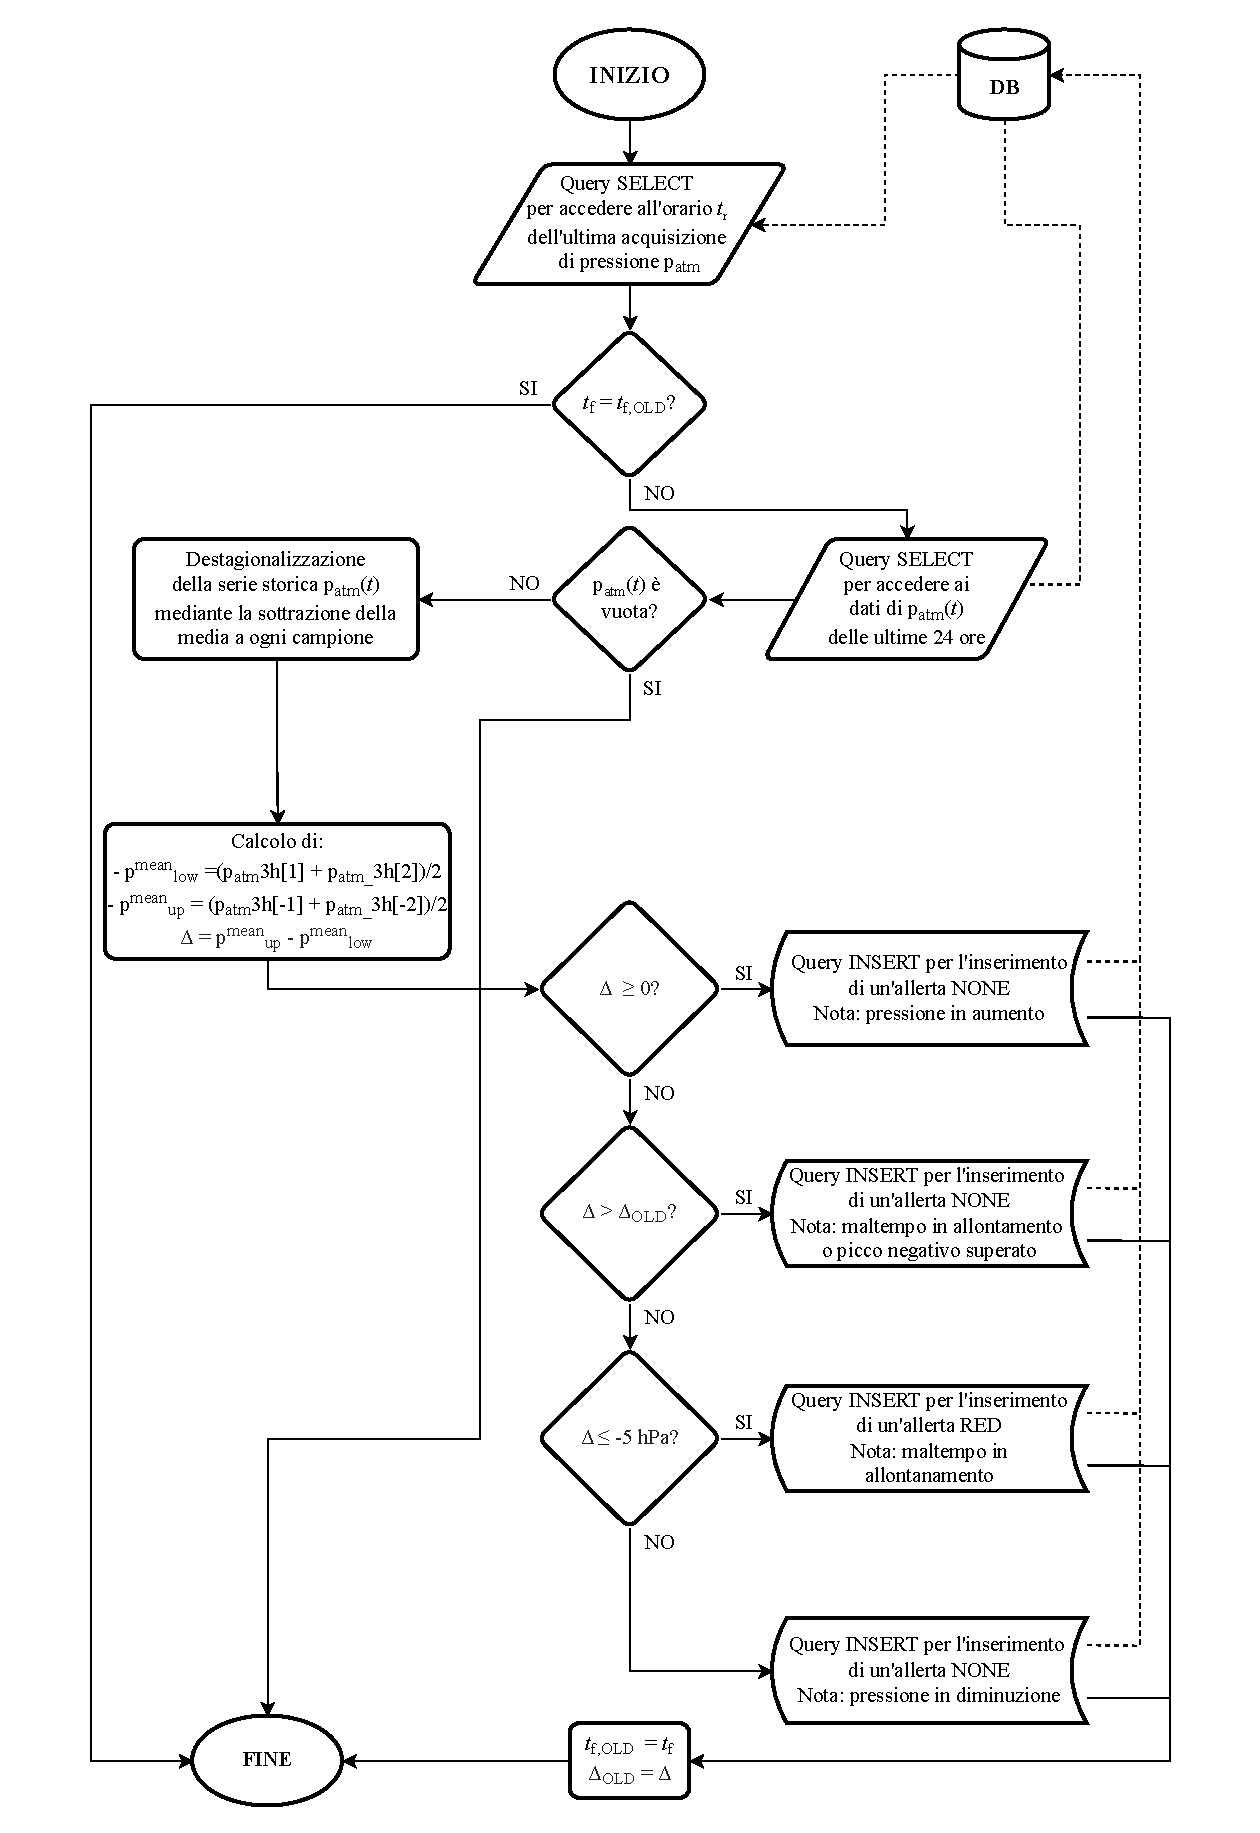
\includegraphics[width=1\linewidth]{./Iterazione 3/OtherFiles/FC - Generatore allerte BW.pdf}
	\caption{diagramma di flusso relativo all'algoritmo di generazione delle allerte maltempo.}
	\label{fig:BFFlowChart}
\end{figure}

\paragraph{Generatore di allerte nebbia e brina}

\subparagraph{Cenni di meteorologia} Per prevedere le formazioni di nebbia e brina è necessario calcolare il \textit{punto di rugiada} $T_d$, ossia la temperatura alla quale l'acqua contenuta nell'aria di un ambiente condensa e si trasforma in gocce d'acqua; esso viene raggiunto quando l'umidità relativa raggiunge il \SI{100}{\percent}, cioè nell'istante in cui l'aria diventa satura e non riesce più a contenere l'umidità ambientale. Il punto di rugiada si determina tramite l'\textit{approssimazione di Magnus-Tetens}:
\[ T_d = \frac{b \cdot \alpha(T,UR)}{a - \alpha(T,UR)}\]
\[\mbox{con } \alpha(T,UR) = \frac{a \cdot T}{b + T} + \ln(UR) \mbox{, } a = \si{17,27} \mbox{ e } b = \si{237,7}\si{\degreeCelsius}\]
\[T\mbox{ (temperatura misurata): } \SI{-20}{\degreeCelsius} < T < \SI{60}{\degreeCelsius}\]
\[UR\mbox{ (umidità relativa): } 0,01 < UR < 1,00\]
La nebbia si forma quando $T = T_d$ e in assenza di vento, mentre la brina quando $T = T_d$ con $T_d < 0$

\subparagraph{Descrizione dell'algoritmo}
\todo{domani sarà ok :-)}

\begin{figure}[h!]
	\centering
	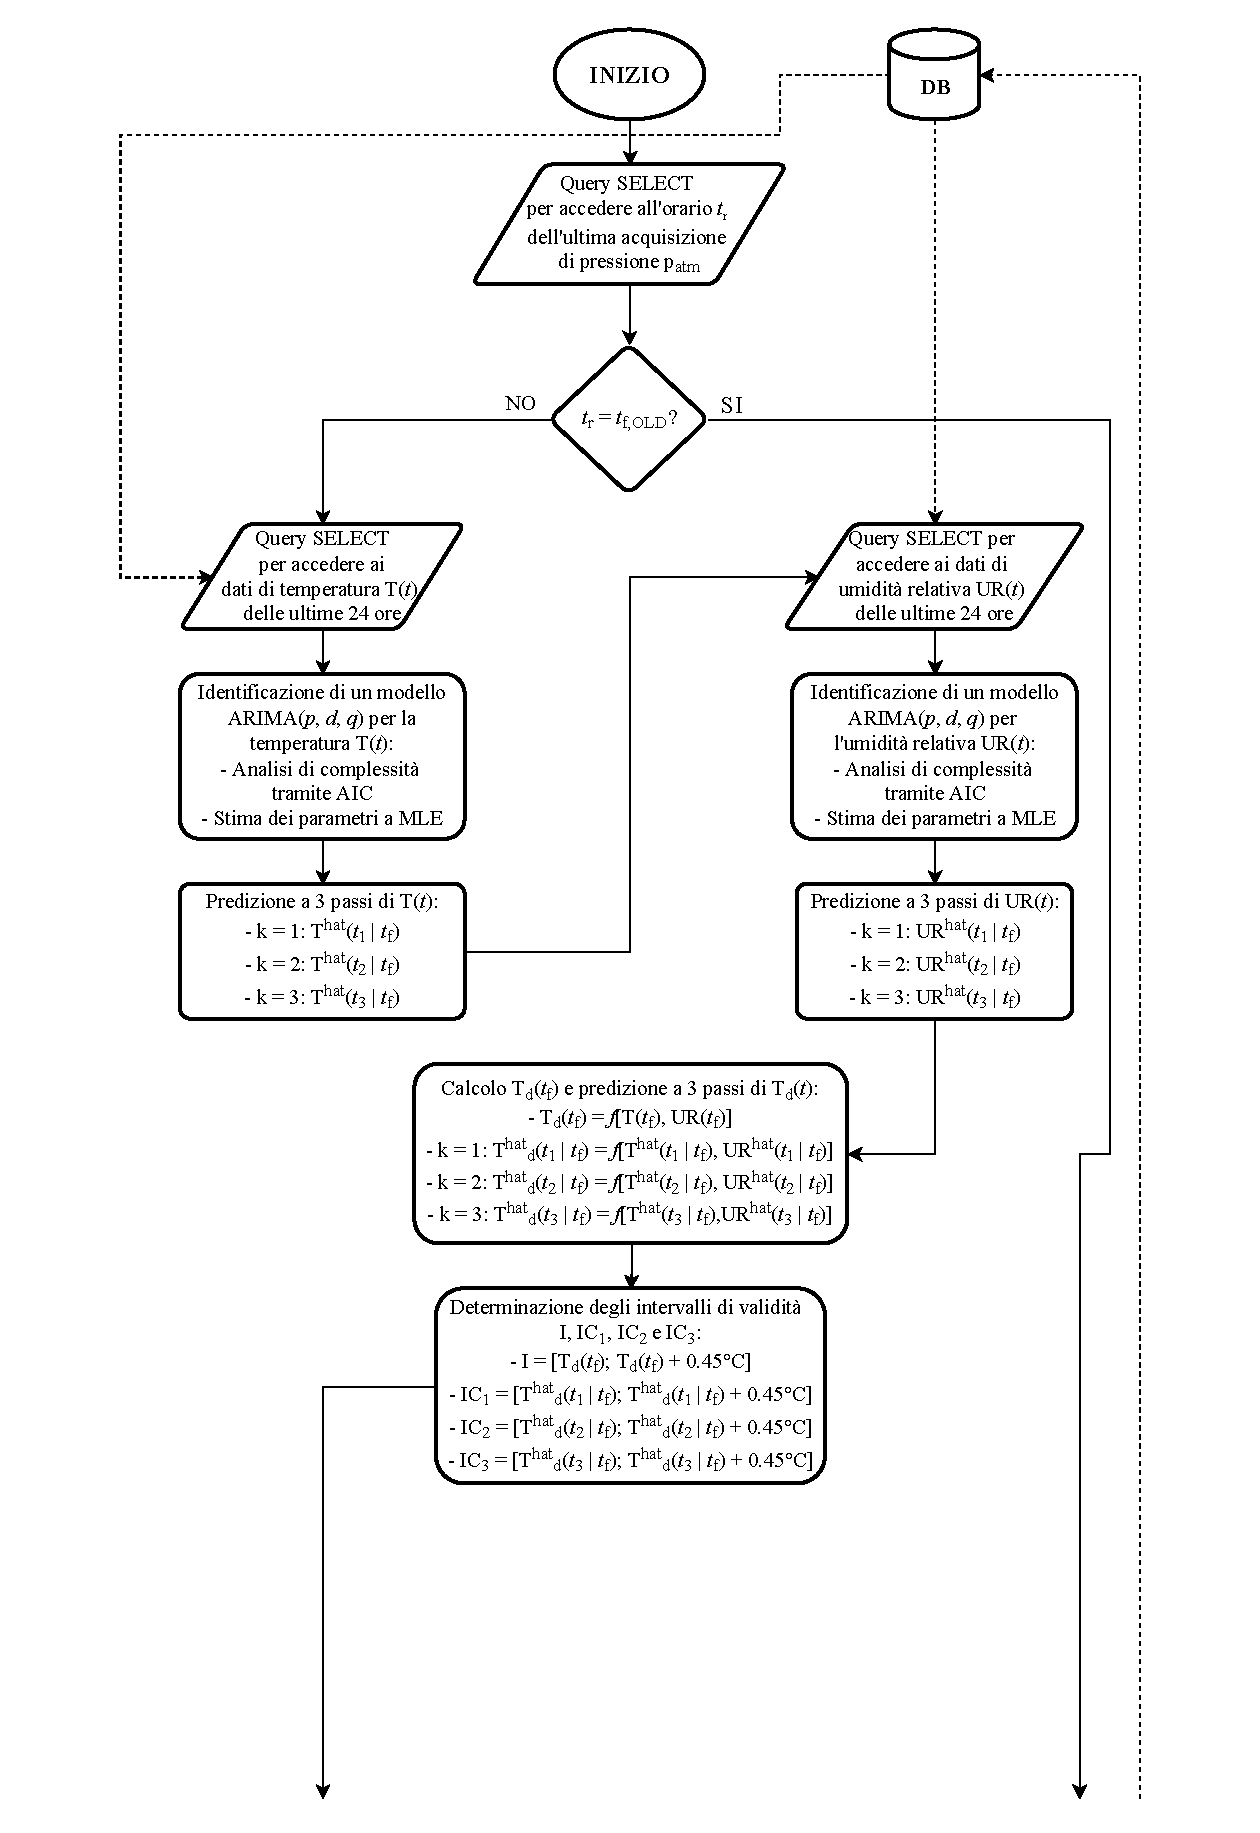
\includegraphics[width=1\linewidth]{./Iterazione 3/OtherFiles/FC - Generatore allerte F&F(1).pdf}
	\caption{diagramma di flusso relativo all'algoritmo di generazione delle allerte nebbia e brina, parte~1.}
	\label{fig:FFFlowChart_1}
\end{figure}

\begin{figure}[h!]
	\centering
	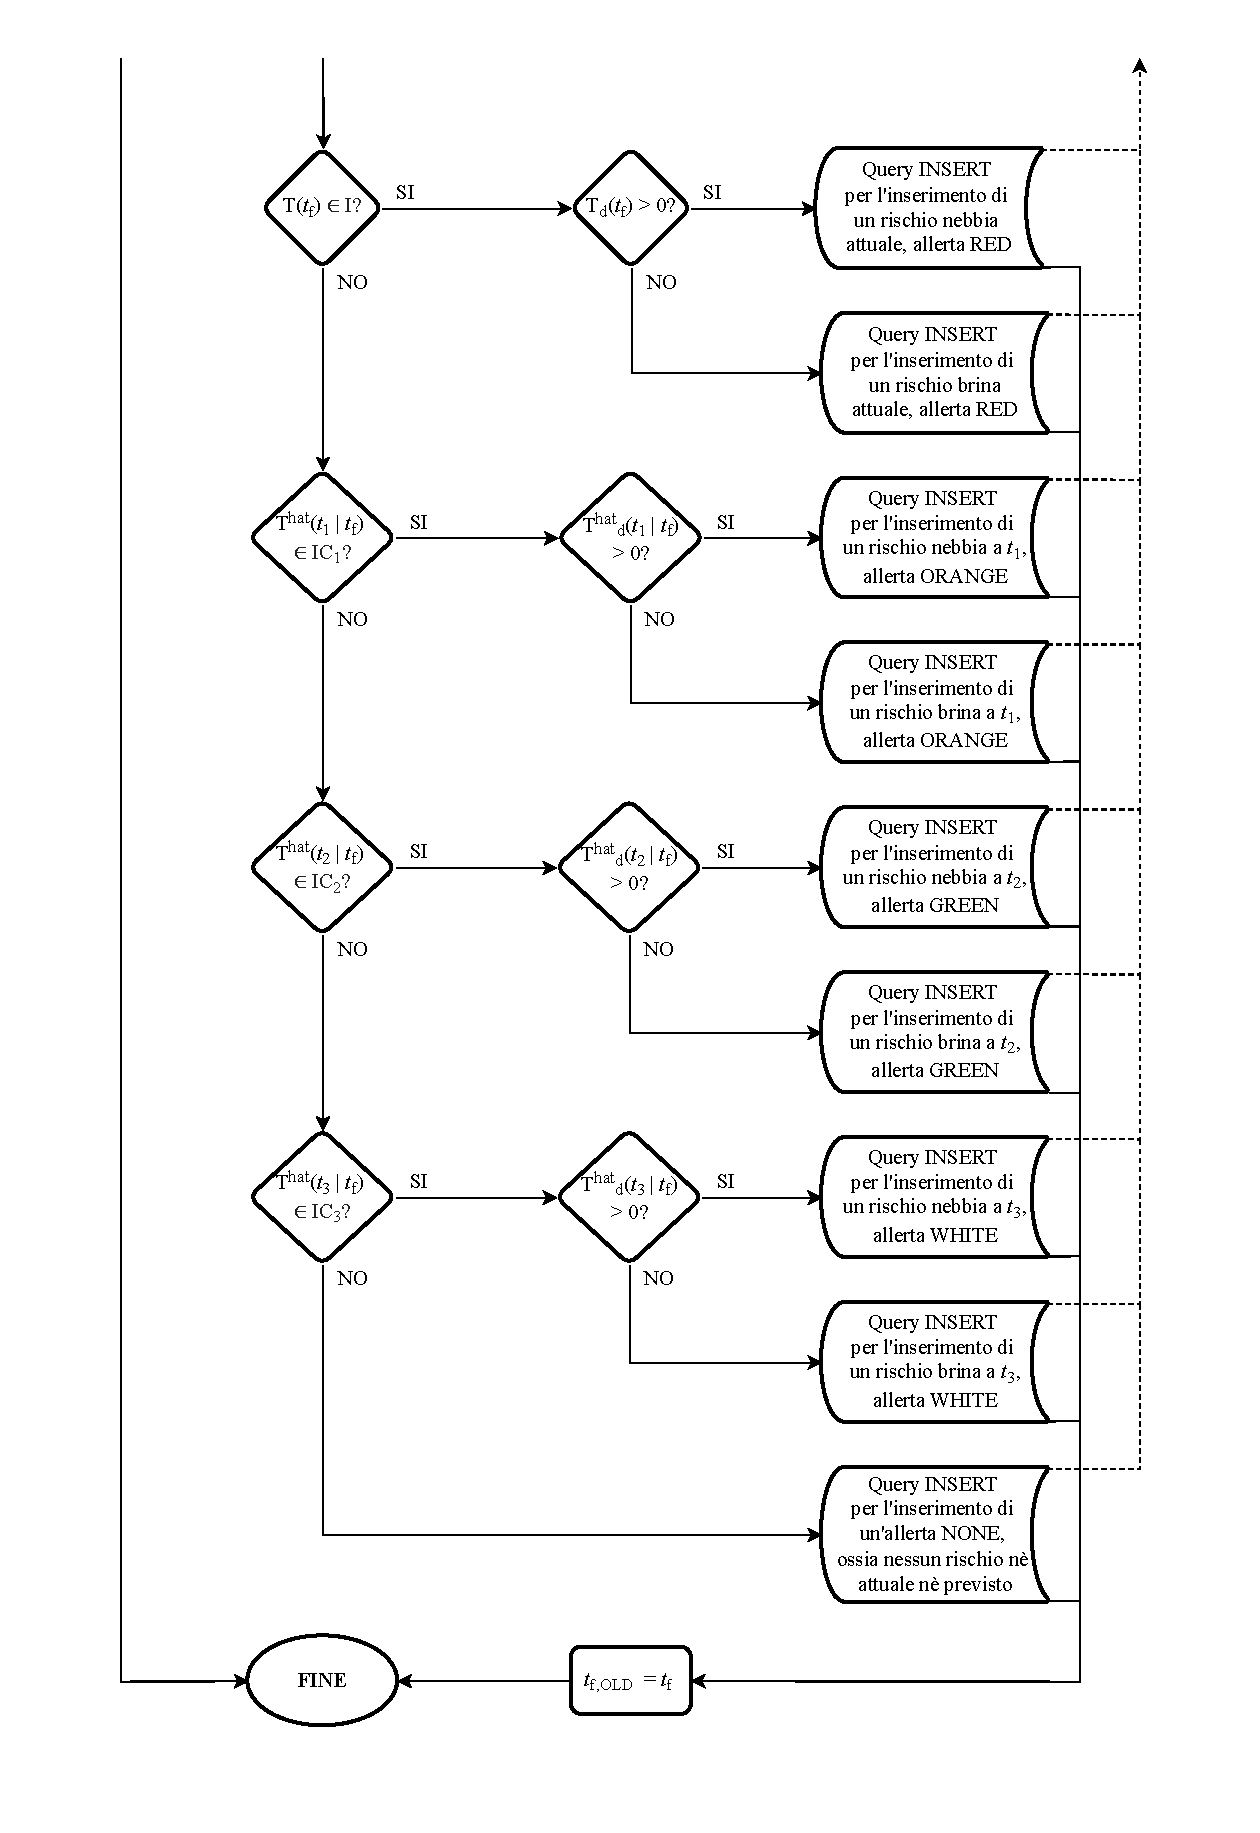
\includegraphics[width=1\linewidth]{./Iterazione 3/OtherFiles/FC - Generatore allerte F&F(2).pdf}
	\caption{diagramma di flusso relativo all'algoritmo di generazione delle allerte nebbia e brina, parte~2.}
	\label{fig:FFFlowChart_2}
\end{figure}